\documentclass[border=4pt,varwidth=17cm]{standalone}
\usepackage{amsmath,amssymb,mathrsfs,mathtools}
\usepackage{tikz}
\usetikzlibrary{positioning,fit,backgrounds,arrows.meta}
\def\RR{{\mathbb R}}\def\eps{\varepsilon}\def\then{\Rightarrow}
\def\J{\mathcal{J}_L}\def\A{\mathcal{A}_{f,g}}\def\Sol{\mathcal{S}_{f,g}}
\def\limsup{\mathop{\overline{\lim}}}\def\liminf{\mathop{\underline{\lim}}}
\def\Of{{\sf (O$_f$)}}\def\Og{{\sf (O$_g$)}}
\def\Rv{{\sf (R$_{\rm v}$)}}\def\Rh{{\sf (R$_{\rm h}$)}}
\begin{document}


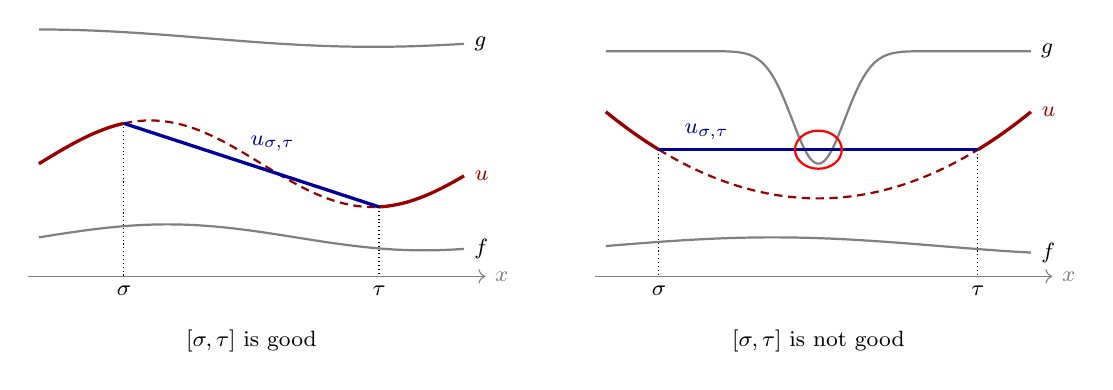
\begin{tikzpicture}[font=\footnotesize]
% left: good interval
\begin{scope}[x=1.35cm, y=1.1cm, declare function={U(\t)=1.3+0.5*sin(deg(1.5*\t)); F(\t)=0.45+0.15*sin(deg(1.3*\t)); G(\t)=2.75+0.1*cos(deg(\t));}]
  \draw[->, gray] (-0.1,0) -- (4.2,0) node[right] {$x$};
  \draw[thick, gray, domain=0:4, samples=80, smooth] plot (\x,{F(\x)}) node[right, black] {$f$};
  \draw[thick, gray, domain=0:4, samples=80, smooth] plot (\x,{G(\x)}) node[right, black] {$g$};
  \draw[very thick, red!60!black, domain=0:0.8, samples=30, smooth] plot (\x,{U(\x)});
  \draw[very thick, red!60!black, domain=3.2:4, samples=30, smooth] plot (\x,{U(\x)}) node[right] {$u$};
  \draw[thick, red!60!black, densely dashed, domain=0.8:3.2, samples=60, smooth] plot (\x,{U(\x)});
  \draw[very thick, blue!60!black] (0.8,{U(0.8)}) -- (3.2,{U(3.2)});
  \node[blue!60!black, above right] at (1.9,{(U(0.8)+U(3.2))/2+0.05}) {$u_{\sigma,\tau}$};
  \draw[densely dotted] (0.8,{U(0.8)}) -- (0.8,0) node[below] {$\sigma$};
  \draw[densely dotted] (3.2,{U(3.2)}) -- (3.2,0) node[below] {$\tau$};
  \node at (2,-0.75) {$[\sigma,\tau]$ is good};
\end{scope}
% right: not good
\begin{scope}[shift={(7.2,0)}, x=1.35cm, y=1.1cm, declare function={V(\t)=0.9+0.25*(\t-2)^2; F(\t)=0.35+0.1*sin(deg(\t)); G(\t)=2.6-1.3*exp(-((\t-2)/0.35)^2);}]
  \draw[->, gray] (-0.1,0) -- (4.2,0) node[right] {$x$};
  \draw[thick, gray, domain=0:4, samples=80, smooth] plot (\x,{F(\x)}) node[right, black] {$f$};
  \draw[thick, gray, domain=0:4, samples=120, smooth] plot (\x,{G(\x)}) node[right, black] {$g$};
  \draw[very thick, red!60!black, domain=0:0.5, samples=30, smooth] plot (\x,{V(\x)});
  \draw[very thick, red!60!black, domain=3.5:4, samples=30, smooth] plot (\x,{V(\x)}) node[right] {$u$};
  \draw[thick, red!60!black, densely dashed, domain=0.5:3.5, samples=60, smooth] plot (\x,{V(\x)});
  \draw[very thick, blue!60!black] (0.5,{V(0.5)}) -- (3.5,{V(3.5)});
  \node[blue!60!black, above] at (0.95,{V(0.5)}) {$u_{\sigma,\tau}$};
  \draw[red, thick] (2,{V(0.5)}) circle (0.22);
  \draw[densely dotted] (0.5,{V(0.5)}) -- (0.5,0) node[below] {$\sigma$};
  \draw[densely dotted] (3.5,{V(3.5)}) -- (3.5,0) node[below] {$\tau$};
  \node at (2,-0.75) {$[\sigma,\tau]$ is not good};
\end{scope}
\end{tikzpicture}


\end{document}
